%% marcel's template

\documentclass[12pt]{article}
\usepackage[margin=0.5in]{geometry}
\usepackage{amsmath,amsthm,amssymb,amsfonts,tikz,tikzsymbols}
\usepackage[shortlabels]{enumitem}

\usepackage{float}% for making figures behave with H

\usepackage{hyperref}
\hypersetup{
  colorlinks   = true,    % Colours links instead of ugly boxes
  urlcolor     = blue,    % Colour for external hyperlinks
  linkcolor    = blue,    % Colour of internal links
  citecolor    = red      % Colour of citations
}

\newenvironment{rcases}
  {\left.\begin{aligned}}
  {\end{aligned}\right\rbrace}

\newcommand{\N}{\mathbb{N}}
\newcommand{\Z}{\mathbb{Z}}
\newcommand{\Q}{\mathbb{Q}}
\newcommand{\R}{\mathbb{R}}
\newcommand{\C}{\mathbb{C}}
\newcommand{\F}{\mathbb{F}}
\newcommand{\RA}{\Rightarrow}
\newcommand\defeq{\mathrel{\stackrel{\makebox[0pt]{\mbox{\normalfont\tiny def}}}{=}}}

\newcommand{\M}{\mathbb{M}}

\renewcommand\qedsymbol{$\Smiley$}

\newenvironment{problem}[2][Question]{\begin{trivlist}
\item[\hskip \labelsep {\bfseries #1}\hskip \labelsep {\bfseries #2.}]}{\end{trivlist}}
\newenvironment{exercise}[2][Exercise]{\begin{trivlist}
\item[\hskip \labelsep {\bfseries #1}\hskip \labelsep {\bfseries #2.}]}{\end{trivlist}}
%If you want to title your bold things something different just make another thing exactly like this but replace "problem" with the name of the thing you want, like theorem or lemma or whatever

\begin{document}
 
%\renewcommand{\qedsymbol}{\filledbox}
%Good resources for looking up how to do stuff:
%Binary operators: http://www.access2science.com/latex/Binary.html
%General help: http://en.wikibooks.org/wiki/LaTeX/Mathematics
%Or just google stuff
 
\title{\texttt{DATA\_SILSO\_HISTO}\\Quality Control Report}
\author{Stephen Fay}
\maketitle

\tableofcontents

\section{Introduction}
\subsection{Github repository and project}
    https://github.com/dcxSt/DATA\_SILSO\_HISTO\_search \\
    https://github.com/users/dcxSt/projects/2?fullscreen=true
    
\subsection{Brief History et Mise en Contexte}

For centuries we have observed the sun and it's ever mysterious sunspots. The 11 year sunspot cycle has long been a subject of debate. Today we wish to have precise quantification of solar activity throughout the previous centuries. This is made possible by the sunspot series. For the past 3 to 4 hundred years people all over the Eurasian continent have been recording the number of sunspots that appear on the sun's earth facing half. 

The aim of this project is to do a quality control of the data in DATA\_SILSO\_HISTO. Once the data is fixed and cleaned up, it will be stored on a new database - temporarily named GOOD\_DATA\_SILSO in a more user-friendly format to what currently exists. I will also get rid of any useless or redundant columns (such as the observers comment column - there are no comments )': ). A third, temporary database will be mad to keep a closer eye on the data that still needs to be examined with more scrutiny : BAD\_DATA\_SILSO. This database will act as intermediary between DATA\_SILSO\_HISTO and GOOD\_DATA\_SILSO. We will effectively be storing 2 databases-worth of information in 3 databases. The original DATA\_SILSO\_HISTO will have the old data and will be corrected in due course. The intermediary BAD\_DATA\_SILSO will start as a copy of DATA\_SILSO\_HISTO and end up empty as the corrected data is removed from it and placed, in the new format, into GOOD\_DATA\_SILSO.


\section{Setup}

\subsection{What do the flags mean?}\label{flags section}
\newpage% idk how to make tables behave!
\begin{table}[h!]
    \centering
    \begin{tabular}{c|c|c|c|c|c|c|c|c|c}
        0 & 1 & 2 & 3 & 4 \\
        same as Null & suspicious & Comment in journal = ? & move to bin & suspiciously high\\
        \hline
        5 & 6 & 7 & 8 & 9\\
        very suspicious & misc see comment & derived from area-measurements & null groups & null sunspots
         
    \end{tabular}
    \caption{Flags key}
    \label{tab:flag}
\end{table}
\begin{enumerate}[start=0]
    \item The default for the flag is NULL, when is estimate that the datapoint is perfect and there is nothing wrong with it, I can put it to zero 0.
    \item If the data looks fishy but I'm not quite sure either what is wrong with it or how wrong it is this is flagged with a 1 - the default.
    \item If in the Mitteilungen journals there is written a `?' next to one of the data points, I will mark it with a 2, this means that the observer is not quite confident in his/her result. See \ref{what is flag 2 question mark} - July 3 for speculation on what I think comment `?' means.
    \item A flag that signifies that this data point is definitely going into the bin
    \item For data that is very dodgy but it is ambiguous as to weather or not it is correct, to determine its validity closer examination is required
    \item For data that is definitely wrong, the difference between 5 and 4 is illustrated by example: if i find that a datapoint has a groups number of 30 I will mark it with a 4 and comment it, because this is suspicious, if a datapoint has a groups number over 60 or above, it will be marked with a 5 (trust me there are some in the hundreds).
\end{enumerate}


\subsection{Equations}

\begin{equation}\label{derivde equation}
    r = a\cdot(10 g + b\cdot f) = 10 a\cdot g + c\cdot f
\end{equation}

\begin{equation}\label{standard deviation equation}
    \sigma = \sqrt{\frac{\sum_{i=1}^{n} (x_i - \bar{x})^2}{n-1}}  \quad \quad \quad \quad 
    var = \frac{\sum_{i=1}^{n} (x_i - \bar{x})^2}{n-1}
\end{equation}

Since we have models where $\bar{x}$ is not the mean but a linear model
\begin{equation}\label{standard deviation percentage equation}
    \sigma\% = 100\cdot \sqrt{\frac{\sum_{i=1}^{n}\big(\frac{x_i-\bar{x}}{\bar{x}}\big)^2}{n-1}}
\end{equation}


\subsection{Python scripts - what they contain}

See README.md


\section{Condensed Log}

\subsubsection{Before The Solstice}
I only started the log on the solstice so I forgot the details of what I was doing before then. The time was spent learning the basics of \texttt{SQL} and how to interface with an \texttt{SQL} database through the mysql terminal; acquainting myself with the data and with what it is I ought to be doing. This is the period where I wrote some of the basic methods that I now use every day for accessing and connecting with the Mittheilungen.

\subsubsection{Friday June 21}
\begin{itemize}
    \item Started writing the log
    \item Made `searching\_the\_manuals.py'
    \item Searching database for `uncertain' comments
\end{itemize}
    
\subsubsection{Monday June 24}
\begin{itemize}
    \item Discovered and sorted a bunch of duplicate data, two data-points for one date and one observer
    \item Methods used can be found in \texttt{searching\_the\_manuals.py}
\end{itemize}
    
\subsubsection{Tuesday June 25}
\begin{itemize}
    \item Backed up the databases and started flagging for the moving process.
    \item Wrote a new script to deal uniquely with deleting the duplicates (and putting them into `\texttt{RUBBISH\_DATA}')
    \item Commented the rubbished duplicate data points
\end{itemize}
    
\subsubsection{Wednesday June 26}
\begin{itemize}
    \item Wrote methods for finer mass commenting (in \texttt{db\_edit.py})
    \item Flagged data with abnormally large groups and or sunspots numbers. (FLAG=4 WHERE $>$ 100 ; FLAG=5 WHERE $>$ 250)
    \item Set 212 flags 3 for putting things in the bin. There are still 4000 pairs of duplicates that need attending to, originally there where 14000
    \item Scrutinised what I had flagged, reread my scripts, checked that things are in the right place.
    \item Having doubts about what is reasonable / unreasonable sunspots number.
\end{itemize}
    
\subsubsection{Thursday June 27}
\begin{itemize}
    \item Scrutinised flagged data from yesterday
    \item Turned my attention to the data labeled `*' in the comments
    \item Moved the flagged duplicates to \texttt{RUBBISH\_DATA}
    \item Found many instances of data written in wrong year
    \item Started writing \texttt{corrections\_needed\_handwritten.txt}, to make clear all my tasks.
\end{itemize}
    
\subsubsection{Friday June 28} 
\begin{itemize}
    \item The notes I took about the duplicates can be found in different\_value\_duplicates.txt, some things I found interesting so I decided to copy most of the file into this report (see long log)
\end{itemize}
    
\subsubsection{Monday July 1}
\begin{itemize}
    \item Using what I did on Friday to bin some duplicated data and modify some other data
    \item Made a new alias in \texttt{DATA\_SILSO\_HISTO} (and \texttt{BAD\_DATA\_SILSO}) called `Brunner Assistent'.
    \item Backed up the the databases to sql files
    \item Most of this data has been cleaned up, the rest can be done by hand
\end{itemize}
    
\subsubsection{Tuesday July 2}
\begin{itemize}
    \item Made some pretty plots in \textit{suspicious sunspots plots.ipynb} in the root directory
    \item Made a method in the jupyter notebook mentioned above that plots an observer's stuff and color codes the flags.
    \item Checked some of them in the journals
    \item Started patching Tacchini's missing holes
\end{itemize}
    
\subsubsection{Wednesday July 3}\label{what is flag 2 question mark}
\begin{itemize}
    \item Continued fixing Tacchini (see figure \ref{fig:tacchini})
    \item Went back to searching the manuals for errors from error sheet. 
    \item Looking through for `uncertain' comments
    \item Figured out what COMMENT=`?' means; blurry image / bad definition of img
    \item Found some comments where there is both an observer and a question mark at the same time, for these ones I left the comments as they are and changed only the flag from 1 to 2.
    \item Finished looking at red comments (I still need to change them and move them all with python, I will do it tomorrow.) 
    \item Looking at blue comments (the ones where comments are just numbers)
    \item Backed up databases
    \end{itemize}
            
\subsubsection{Thursday July 4}
\begin{itemize}
    \item Looking into Carrington's case.
    \item I updated the flag 7 to ``derived from area-measurement" and flagged all of Secchi's sunspot values that were derived from the penumbra and / or umbra.
    \item Dealt with Secchi
    \item Spoke to F. Clette about the possible conversion from the `aire' to a sunspots number. He gave me some clues as to where to look in the mitt.
    \item Excitement! I found on page 131 of Mitt 31-40 written after rubrics 299 a description of how the author (I think R. Wolf himself) derived a formula for turning Secchi's `aire' into a sunspots number
    \item \ref{converting the `aire'} here is what is written in German and Italian, with a translation in English.
    \item Backed up databases
\end{itemize}
        
\subsubsection{Friday July 5}
\begin{itemize}
    \item Continued working on Carrington
\end{itemize}

\subsubsection{Monday July 8}
\begin{itemize}
    \item Finished deriving Carrington
    \item Backed up databases
\end{itemize}

\subsubsection{Tuesday July 9}
\begin{itemize}
    \item Derived Kew's misbehaving data
    \item Made a new `README.md' that auto-generates based on what is inside my python scripts
    \item Tidied the report and added some figures
\end{itemize}



\section{Tables & Figures}

\subsubsection{The original sql data tables format}

\begin{table}[h!]
    \centering
    \caption{DESCRIBE DATA}
    \begin{tabular}{c|c|c|c|c|c}% l c r = Left Centre Right
        \textbf{Field} & \textbf{Type} & \textbf{Null} & \textbf{Key} & \textbf{Default} & \textbf{Extra}  \\
        \hline
        ID & int(11) & No & PRI & NULL & auto\_increment \\
        
        DATE & date & YES && NULL & \\
        
        FK\_RUBRICS & int(11) & YES & MUL & NULL &  \\
        
        FK\_OBSERVERS & int(11) & YES & MUL & NULL &  \\
        
        GROUPS & int(11) & YES && NULL &  \\
        
        SUNSPOTS & int(11) & YES && NULL & \\
        
        WOLF & int(11) & YES && NULL &  \\
        
        QUALITY & int(11) & YES && NULL &  \\
        
        COMMENT & text & YES && NULL &  \\
        
        DATE\_INSERT & datetime & YES && NULL &  \\
        
        FLAG (i added this) & tinyint(1) & YES && NULL &  \\
        
    \end{tabular}
    \label{tab:data-og}
\end{table}

\begin{table}[h!]
    \centering
    \caption{DESCRIBE OBSERVERS}
    \begin{tabular}{c|c|c|c|c|c}% l c r = Left Centre Right
        \textbf{Field} & \textbf{Type} & \textbf{Null} & \textbf{Key} & \textbf{Default} & \textbf{Extra}  \\
        \hline
        ID & int(11) & NO & PRI & NULL & auto\_increment \\
        
        ALIAS & varchar(50) & YES && NULL & \\
        
        FIRST\_NAME & varchar(50) & YES && NULL &  \\
        
        LAST\_NAME & varchar(50) & YES && NULL &  \\
        
        COUNTRY & varchar(50) & YES && NULL &  \\
        
        INSTRUMENT & varchar(50) & YES && NULL & \\
        
        COMMENT & text & YES && NULL &  \\
        
        DATE\_INSERT & datetime & YES && NULL &  \\
        
    \end{tabular}
    \label{tab:data-og}
\end{table}

\begin{table}[h!]
    \centering
    \caption{DESCRIBE RUBRICS}
    \begin{tabular}{c|c|c|c|c|c}% l c r = Left Centre Right
        \textbf{Field} & \textbf{Type} & \textbf{Null} & \textbf{Key} & \textbf{Default} & \textbf{Extra}  \\
        \hline
        RUBRICS\_ID & int(11) & NO & PRI & NULL & auto\_increment \\
        
        RUBRICS\_NUMBER & int(11) unsigned & NO && NULL & \\
        
        MITT\_NUMBER & int(11) unsigned & NO && 0 &  \\
        
        PAGE\_NUMBER & int(11) unsigned & YES && NULL &  \\
        
        SOURCE & text & NO && NULL &  \\
        
        SOURCE\_DATE & date & YES && NULL & \\
        
        COMMENTS & text & YES && NULL &  \\
        
        DATE\_INSERT & datetime & YES && NULL &  \\
        
        NB\_OBS & int(11) & YES && NULL & \\
        
    \end{tabular}
    \label{tab:data-og}
\end{table}

\newpage{}

\subsubsection{My new sql data table format}

\begin{table}[h!]
    \centering
    \caption{DESCRIBE DATA (the only table)}
    \begin{tabular}{c|c|c|c|c|c}% l c r = Left Centre Right
        \textbf{Field} & \textbf{Type} & \textbf{Null} & \textbf{Key} & \textbf{Default} & \textbf{Extra}  \\
        \hline
        ID & int(11) unsigned & No & PRI & NULL & auto\_increment \\
        
        DATE & date & YES && NULL & \\
        
        GROUPS & int(11) & YES && NULL &  \\
        
        SUNSPOTS & int(11) & YES && NULL & \\
        
        WOLF & int(11) & YES && NULL &  \\
        
        COMMENT & text & YES && NULL &  \\
        
        DATE\_INSERT & datetime & YES && NULL &  \\
        
        OBS\_ALIAS & varchar(50) & YES && NULL & \\
        
        FIRST\_NAME & varchar(50) & YES && NULL & \\
        
        LAST\_NAME & varchar(50) & YES && NULL & \\
        
        COUNTRY & varchar(50) & YES && NULL & \\
        
        INSTRUMENT\_NAME & varchar(50) & YES && NULL & \\
        
        RUBRICS\_NUMBER & int(11) & YES && NULL & \\
        
        MITT\_NUMBER & int(11) & YES && NULL & \\
        
        PAGE\_NUMBER & int(11) & YES && NULL & \\
        
        FLAG & tinyint(1) unsigned & YES && NULL &  \\
        
        RUBRICS\_SOURCE & text & YES && NULL & \\
        
        RUBRICS\_SOURCE\_DATE & date & YES && NULL & \\
        
    \end{tabular}
    \label{tab:data-og}
\end{table}





\newpage{}

\subsubsection{Figures - plots and graphs}

\begin{figure}[H]
    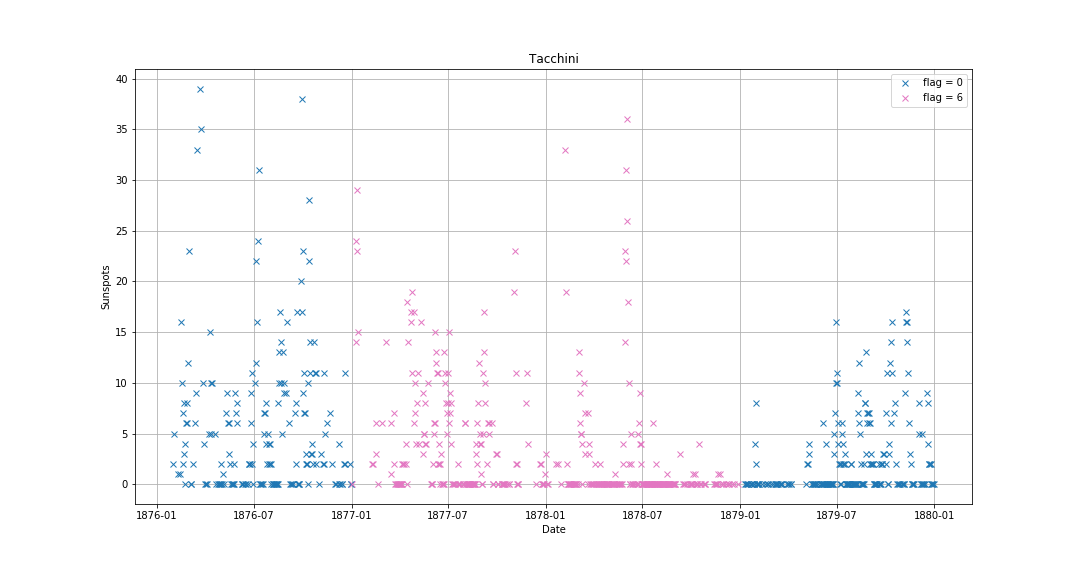
\includegraphics[width=0.5\linewidth]{tacchini1877_patch.png}
    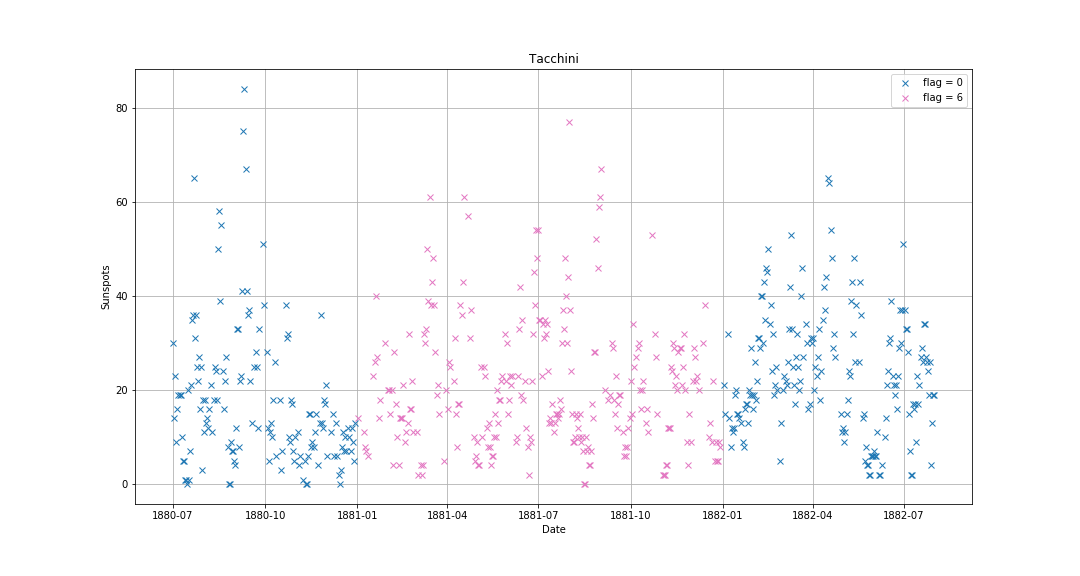
\includegraphics[width=0.5\linewidth]{tacchini1881_patch.png}
    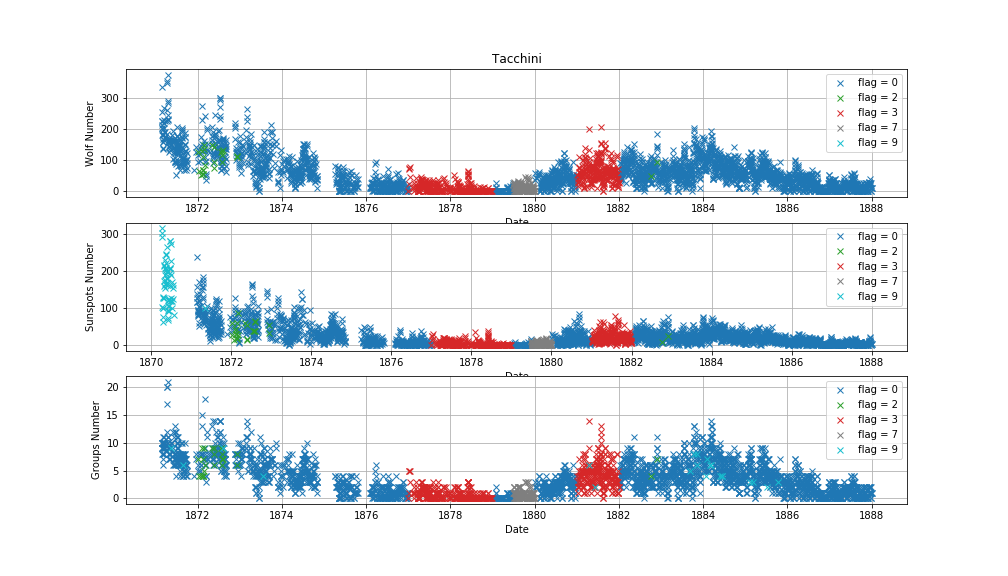
\includegraphics[width=\linewidth]{tacchini_pached.png}
    \caption{Tacchini}
    \label{fig:tacchini}
\end{figure}

\begin{figure}[H]
  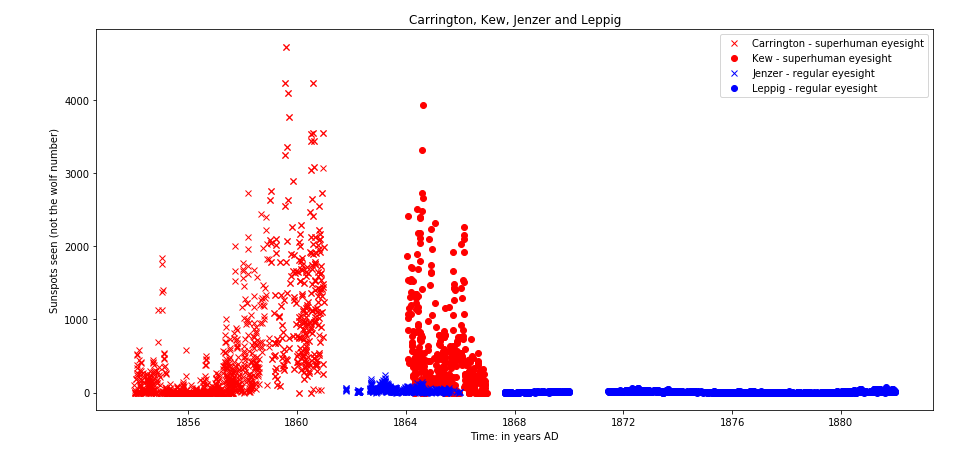
\includegraphics[width=\linewidth]{CarringtonHasGoodEyesight.png}
  \caption{Carrington and Kew - input penumbras instead of sunspots}
  \label{fig:carrington-kew-penumbras}
\end{figure}

\begin{figure}[H]
    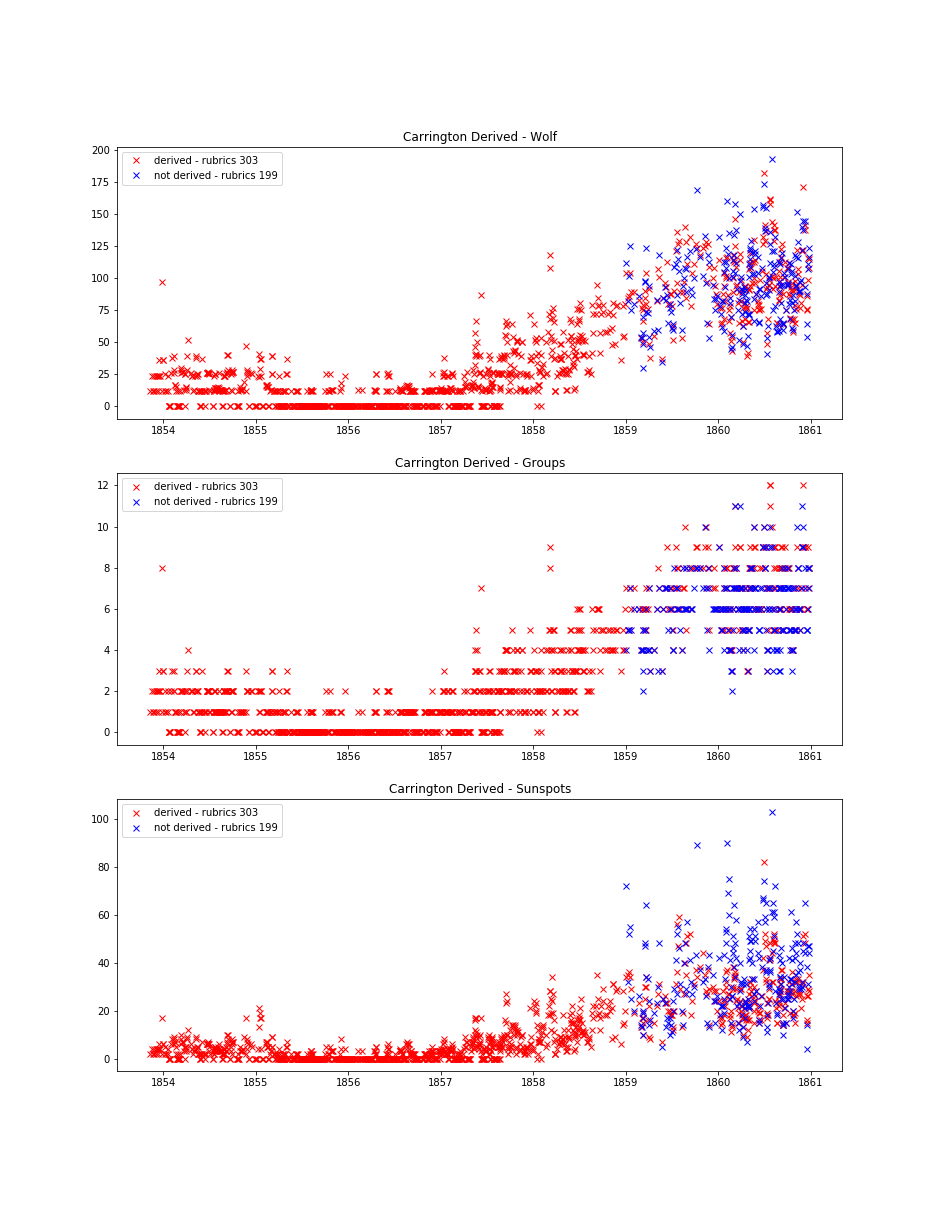
\includegraphics[width=\linewidth]{carrington_derived.png}
    \caption{Carrington derived}
    \label{fig:carrington_derived}
\end{figure}

\begin{figure}[H]
    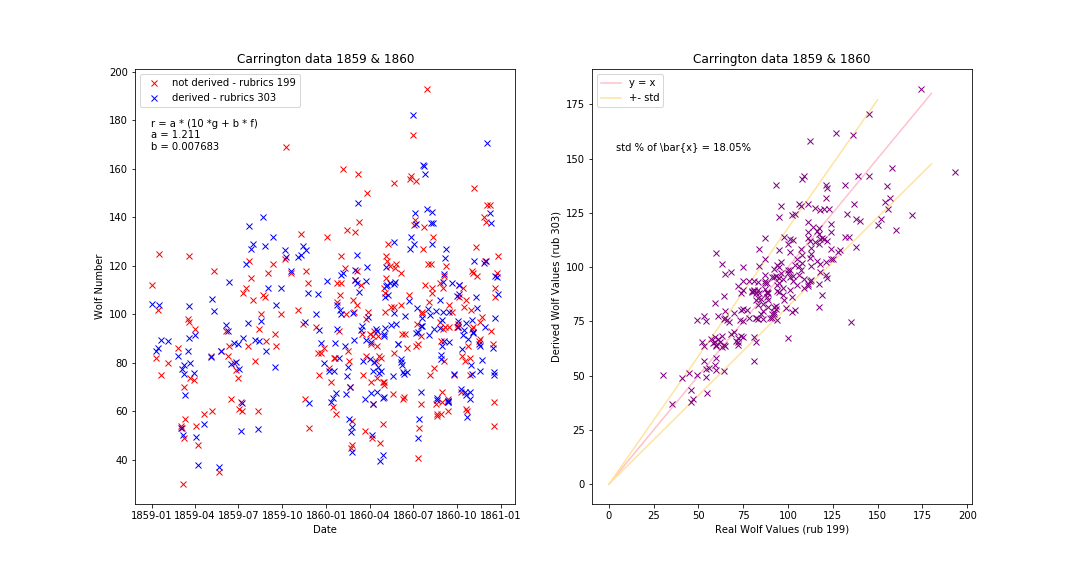
\includegraphics[width=\linewidth]{carrington_fit_wolf.png}
    \caption{Carrington wolf fit}
    \label{fig:carrington_fit_wolf}
\end{figure}

\section{Conclusions}

\subsection{Before and After - outline of the modifications I made to the database}

\subsection{Problems that remain with the database}

This idea will probably never come to fluition - in the spirit of Herr Wolf who was the first one to estimate $\pi$ by monte-carlo approximation, find the frequency of random errors in the Mittheilungen by Monte-Carlo approximation (should take about 1 day). Pick 1000 to 2000 datapoints at random using some algorythem, and find each one in the mittheilungen to see if it is entered correctly, do some stats on this and calculate a student error factor. (better to look up if there are known numbers for this kind of task)

\section{Miscellaneous}

\subsubsection{Thought repository - ideas that may or may not come into fluition depending on how efficiently I work and get things that need to be done done}
\begin{itemize}
    \item make some data visualisations to compare each observer's primary and secondary observing equipment
    \item for each day / month / year find the highest observation and the lowest observations and add it to the graph so that we have like an upper bound and a lower bound. 
    \item figure out how to smooth graphs with matplotlib and make something nice out off the big mess i currently have
    \item pie chart of observers with their number of observations
    \item in the final sunspots number graph cut it into 3 or 4 sections that mark changes in the theory behind sunspots: before wolf ; time where plato's ideas of the sun being a perfect sphere still were around ; 1908 George Ellery Hale discovers the magnetic link (p14 of nature's 3rd cycle) ; 1955 eugene parker's theory (p19 of nature's 3rd cycle) ; Nasa send their probe to near the sun
\end{itemize}

\subsection{Converting the $f$ (`aire')}\label{converting the `aire'}

\subsubsection{rubrics 299, mitt 33, p 128 observer Secchi}\label{rubrics 299, secchi}\\

\textbf{German}
p128) Als Anhang ist ein ``[It] Registro della macchie solarie osservate alla specola del Collegio Romano durante l'anno 1871" gegeben, welches die an einer Reihe von Tagen von Rom. Remiddi gezahlten Gruppen, anstatt der Anzahlder Flecken aber Zahlen enthalt, welche die von ihnen eingenomene Flache in Quadrat-Millimeter angenommen. Ich gebe dieselben in der gewohnten Weise, d. h so, dass die erste Zahl wie immer der Anzahl der Gruppen, die zweite aber jener Flachenzahl entspricht, - die der letztern gleichgesetzte Zahl endlish eine aus ihr nach untenstehender Formel berechnete, der Fleckenzahl moglichst entsprechende Zahl.\\

\textit{Secchi's Data from rubrics 299}\\

p 130) Meine Relativzahlen basiren bekanntlich auf der Annahme, dass die Fleckenthatigkeit zunachst in der Anzahl der Gruppen, in untergeordneter Weise aber auch in der Grosse derselben ein Maass finde, und es wurde dieser Grosse von mir nur darum die Gesammtanzahl der Flecken substituirt, weil ich einerseits durch viele betreffend Vergleichungen gefunden hatte, das mit der Grosse der Hauptflecken meistens auch die Anzahl ihre Begleiter zunehem, also die Anzahl der Flecken annahernd jener Grosse proportional sei, - und es anderseits nicht nur zu zeitraubend fand diese Grosse fortwahrend zu messen, und (was bei den obigen Beobachtungen, welche nur die scheinbaren Flachen geben, wenigstens vorlaufig unterlassen wurde) auf ihr wahres Mass zu reduciren, sondern namentlich auch ein fur altere Beobachtungsreihen (denen sich gewohnlich die Anzahl der Flecken mit ziemlicher Sicherheit, die Grosse dagegen selten auch nur irgendwie annahernd entnehmen lasst) ebenfalls brauchbares Verfahren einfuhren musste. - Die in der obigen Reihe fur viele Tage, and welchen ich selbst Fleckenzahlungen gemacht, und daraus die Relativzahlen $r$ berechnet hatte, gegebenen Flachen haben mir nun die Moglichkeit verschafft die Richtigkeit meines Verfahrens neuerdings zu prufen, und zugleich eine bestimmte Regel aufzustellen, um zur Erganzung meiner Register fur einzeln Tage ause den bestimmten Flachen die fur mich nothigen Fleckenzahlen annahernd zu berchnen: Bezeichne ich namlich die Anzahl der in Rom gezahlten Gruppen mit $g$, die bestimmte Flache aber mit $f$, so muss unter Voraussetzung der Richtigkeit meiner Annahme annahernd fur jeden gemeinschaftlichen Beobachtungstag eine Gleichung
$$r = a\cdot (10 g + b \cdot f) = 10 a \cdot g + c \cdot f$$
bestehen, wo a, b und c constante Factoren sind. Ich bildete nun 120 solcher Gleichungen, ordnete dieselben nach r, nahm je aus 20 das Mittel, und erhielt so die 6 Normalgleichungen \\

{\centering
    \begin{tabular}{c|c|c|c}
    
         & $r = 10 a \cdot g + c\codt f$ & $r'$ & $r - r'$ \\
         \hline
         1 & $60 = a \cdot 37 + c \cdot 46$ & $62$ & $-2$ \\
         2 & $80 = a\cdot 46 + c\cdot 61$ & $78$ & $+2$ \\
         3 & $100 = a\cdot 60 + c\cdot 112$ & $109$ & $-9$ \\
         4 & $120 = a\cdot 63 + c\cdot 117$ & $114$ & $+6$ \\
         5 & $140 = a\cdot 78 + c\cdot 155$ & $143$ & $-3$ \\
         6 & $160 = a\cdot 85 + c\cdot 187$ & $159$ & $+1$ \\
         \hline
         & Mittlere Abweichung && \pm{5}
    \end{tabular}
\par}
aus welchen ich nach der Methode der kleinsten Quadrate 
$$a=1.41 \quad c=0.21 \quad \text{sodann}\ b=0.15$$
und somit fur die romischen Beobachtungen die Reductionsgleichung
$$r' = 1.41(g\cdot 10 + f\codt 0.15)$$
fand. Setze man in die Normalgleichungen diese Werthe fur a und c ein, so erhalt man die ihnen beigeschriebenen r', deren Vergleichung mit den r eine unerwartet gute Uebereinstimmung zeigt. Es hat also diese kleine Untersuchung die Berechtigung des von mir fur die Berechnung der Relativzahlen aufgestellten Principes in schonster Weise bestatigt, und mich anderseits ermuthigt in der obigen Beobachtungsreihe jeder Flache die nach der eben aufgefuhrten Formel berechnete Fleckenzahl beizuschreiben, - wobei ich naturlich in den paar Fallen, wo eine ganz geringe Flache eine Fleckenzahl ergab, welche kleiner als die Gruppenzahl war fur sie diese Gruppenzahl substituirte.\\

\textbf{English} (using \href{http://deepl.com/}{deepl translator})
p128) As appendix is given a ``Register of sunspots observed in the mirror of the Roman College during the year 1871", which is the one on a series of days of Rome. Remiddi paid groups, instead of number spots but contains numbers which assume the area in square millimeters inscribed by them. I give them in the usual way, i.e. in such a way that the first number corresponds, as always, to the number of groups, the second, however, to that number of flats, - which endlessly calculates from the latter equated number a number which corresponds as closely as possible to the number of spots, according to the formula below.\\

\textit{Secchi's Data from rubrics 299}\\

p 130) As is well known, my relative numbers are based on the assumption that the number of spots finds a measure first of all in the number of groups, but in a subordinate way also in the size of the same, and this size was only substituted by me for the total number of spots, because on the one hand I had found by many comparisons that with the size of the main spots mostly also the number of their companions increases, so the number of spots is approximately proportional to that size, - and on the other hand not only too time-consuming was it found to measure these large ones continuously, and (what was at least temporarily omitted in the above observations, which only give the apparent flat ones) to reduce them to their true measure, but especially also to introduce a procedure useful for older series of observations (from which usually the number of spots is quite certain, but the large ones, on the other hand, can seldom be taken out even approximatively) likewise. - The surfaces given in the above series for many days, on which I had made spot payments myself, and had calculated the relative numbers $r$ from them, have now given me the possibility to check the correctness of my method recently, and at the same time to establish a certain rule in order to approximate the numbers of spots necessary for me to supplement my registers for individual days from the certain surfaces: If, for example, I designate the number of groups paid in Rome with $g$, but the certain area with $f$, then, assuming my assumption is correct, an approximate equation must be given for each common observation day
$$r = a\cdot (10 g + b \cdot f) = 10 a \cdot g + c \cdot f$$
where a, b and c are constant factors. I now formed 120 such equations, arranged them according to r, took the mean from each 20, and thus obtained the 6 normal equations \\

{\centering
    \begin{tabular}{c|c|c|c}
    
         & $r = 10 a \cdot g + c\cdot f$ & $r'$ & $r - r'$ \\
         \hline
         1 & $60 = a \cdot 37 + c \cdot 46$ & $62$ & $-2$ \\
         2 & $80 = a\cdot 46 + c\cdot 61$ & $78$ & $+2$ \\
         3 & $100 = a\cdot 60 + c\cdot 112$ & $109$ & $-9$ \\
         4 & $120 = a\cdot 63 + c\cdot 117$ & $114$ & $+6$ \\
         5 & $140 = a\cdot 78 + c\cdot 155$ & $143$ & $-3$ \\
         6 & $160 = a\cdot 85 + c\cdot 187$ & $159$ & $+1$ \\
         \hline
         & Mittlere Abweichung && \pm{5}
    \end{tabular}
\par}

from which I can draw the least squares 
$$a=1.41 \quad c=0.21 \quad \text{sodann}\ b=0.15$$
and therefore for the Roman observations the reduction equation
$$r' = 1.41(g\cdot 10 + f\codt 0.15)$$
found. If one enters this value for a and c in the normal equations, one obtains the r' attributed to them, whose comparison with the r shows an unexpectedly good agreement. So this small examination confirmed in the best way the validity of the principle I had established for the calculation of the relative numbers, and on the other hand it encouraged me in the above series of observations to attribute to each surface the number of spots calculated according to the just listed formula, - whereby I naturally substituted this group number in the few cases where a very small surface resulted in a number of spots which was smaller than the group number for it.

\subsubsection{rubrics 303, mitt 35, p 241 observer Carrington}\label{rubrics 303, carrington}\\

303) Warren De La Rue, Balfour Stewart and Benjamin Loewy, Researches on Solar Physics. Second Series: Area measurements of the Sun-Spots observed by Carrington during the seven Years from 1854 - 1860 inclusive, and deductions therefrom. London 1866 in 4.\\

\textbf{German}
Ich ziehe aus dieser Abhandlung unter fortwahrender Berucksichtigung der unter 199 besprochenen Werkes von Carrington und der unter 129 aufgeguhrten schriftlichen Mittheilung derselben folgende Beobachtungen in der altgebohnten Form, nur dass die der Gruppenzahl folgende Zahl (analog wie bei den unter 299 aufgeguhrten Beobachtungen Secchis) nicht die Anzahl der Flecken, sondern die in Millionsteln der sichtbaren Sonnenhemisphare ausgedruckte Flache derselben Bezeichnen:\\

Durch Vergleichung der fur 1859 und 1860 gegebenen Flachenzahlen mit den in Nr. 199 von Carrington selbst fur dieselben Jahre und Tage mir mitgetheilten Fleckenzahlen, erhalt man, dass durchschnittlich 1000 Flacheneinheiten 24 Flecken entsprechen, und es darf dieses Verhaltniss ohne Anstand benutzt werden, um fur die wenigen Tage, wo das Fleckenregister durch Carrington'sche Beobachtungen erganzt werden kan, die Flachen in Flecken umzusetzen.\\

\textbf{English}
I deduce from this treatise, taking into account the work of Carrington discussed under 199 and the written communication of the same discussed under 129, the following observations in the old-bored form, only that the number following the group number (analogous as in the observations of Secchi examined under 299) does not denote the number of spots, but the area of the same printed out in millionths of the visible solar hemispheres:\\

What follows is observations made by Carrington for the years specified with `aire' numbers instead of sunspots numbers. [it seems someone had the same idea as me]\\

By comparing the surface numbers given for 1859 and 1860 with the spot numbers given in No. 199 by Carrington himself for the same years and days, one obtains that on average 1000 surface units correspond to 24 spots, and this relationship may be used without decency to convert the surfaces into spots for the few days when the spot register can be supplemented by Carrington's observations.

\subsubsection{Rubrics 199, mitt 11-20, p224}

Observations of the Spots on the Sun from 1853 XI 9 to 1861 III 24 made ad Redhill by R. Chr. Carrington. London 1863 (248 Pag., 166 Plat.) in 4.\\

\textbf{German} 
Dieses Ausgezeichnete, erst kurzlich nach Verdienen von der Pariser-Academie mit dem Lalande-Preise bedachte Werk meines verehrten Freundes erlaubt nach seiner Natur kaum einen Auszug, sondern ist zunachst als eine unerschopfliche Fundgrube zu betrachten, in der diejenigen Astronomen, welche sich speqiell mit der Vertheilung der Sonnenflecken, ihren Ortsveranderungen etc. Befassen, ein reiches Material an Zahlen unde Zeichnungen erheben konnen, - wie ja bereits oben eine darauf gegrundete Studie von Herrn Fritz mitgetheilt worden ist, wahrend eine die `Concluding Section' betreffende Arbeit von mir in einer der nachsten Mittheilungen folgen wird. Dagegen mogen hier anhangsweise zur Erganzung der Nr. 129 der Litteratur die Fleckenzahlungen in den Jahren 1859 und 1860 nachgetragen werden, welche mir Herr Carrington seiner Zeit mittheilte, und die ich in der letzten Zeit neuerdings bei Ermittlung der mehrfach erwahnten 5 taggigen Mittel benutzte. Es sind Folgende:\\

\textbf{English}
This excellent work of my esteemed friend, which was awarded the Lalande Prize by the Paris Academy only shortly after it had been earned, hardly permits an excerpt by its nature, but is first to be regarded as an inexhaustible treasure trove in which those astronomers who are particularly concerned with the distribution of sunspots, their changes of place, etc., can be found. As already above a study based on it has been shared by Mr. Fritz, while a work of mine concerning the 'Concluding Section' will follow in one of the next communications. On the other hand, to supplement the No. 129 of the Litteratur, the stain payments in the years 1859 and 1860, which Mr. Carrington informed me of his time and which I recently used in the determination of the repeatedly mentioned 5-day means, may be added here as an appendix. They are the following:


\end{document}





